
Two graph calculi meet on the boundary of configuration space.  The
ordered bar differential is built from Arnold logarithmic forms
$\eta_{ij}=d\log(z_i-z_j)$ and collision residues on
Fulton--MacPherson strata; perturbative field theory is built from
Wick contraction kernels and local vertices.  The error is to identify
these kernels.  The theorem shared by the two calculi is the
stable-graph decomposition of the universal MC element.

For the Heisenberg algebra $\mathcal{H}_{\kappa^{\mathrm{Heis}}}$,
the double-pole OPE gives the Gaussian BV/bar comparison for free
fields (Proposition~\ref{prop:bar-bv-free-fields}) and the explicit
higher-genus bar cohomology of Theorem~\ref{thm:heisenberg-higher-genus}.
Conjecture~\ref{conj:v1-bar-cobar-path-integral-heisenberg} asks for the
all-genera comparison map, not for an equality of the Wick kernel with
$\eta_{ij}$.  For interacting chiral algebras, Volume~I proves the
genus-$0$ BRST/bar quasi-isomorphism on the anomaly-free locus
(Theorem~\ref{thm:brst-bar-genus0}) and the local binary/ternary
reduction package; the all-genera perturbative comparison is
Conjecture~\ref{conj:v1-bar-cobar-path-integral}.  The
Feynman--bar mnemonic (Remark~\ref{rem:feynman-bar-bridge}) is therefore
a controlled dictionary: Arnold form $=$ logarithmic collision form,
vertex $=$ chiral residue, boundary stratum $=$ stable-graph gluing.
It is not a loop$=$genus identity.

\begin{construction}[Feynman transform as stable-graph MC decomposition]
\label{constr:feynman-stable-graph}
\index{Feynman transform!stable-graph decomposition|textbf}
\index{stable graph!MC decomposition|textbf}
\index{MC element!stable-graph sum}
\textup{(}\emph{quadrant} Open, \emph{presentation} bar / twisting
coalgebra in modular Feynman transform of $\mathrm{FCom}$,
\emph{level} 2 of the Beilinson tower with descent to clutching at
level~$5$, \emph{hypothesis package} Getzler--Kapranov modular
operad on $\overline{\mathcal{M}}_{g,n}$; finite stable-graph index
set $\mathsf{Gr}^{\mathrm{st}}_{g,n}$ at fixed $(g, n)$; the
$\Theta_\cA$ is the modular MC element of
Theorem~\ref{thm:explicit-theta}.\textup{)}
The Feynman transform $\mathrm{FT}(\mathrm{FCom})$ of the commutative modular operad decomposes the MC element $\Theta_\cA$ as a stable-graph sum:
\[
\Theta_\cA^{(g,n)} = \sum_{\Gamma \in \mathsf{Gr}^{\mathrm{st}}_{g,n}} \frac{1}{|\mathrm{Aut}(\Gamma)|} \cdot W_\Gamma(\cA),
\]
where $W_\Gamma(\cA)$ is the $\Gamma$-amplitude of
Construction~\ref{constr:stable-graph-decomposition}.  The displayed
sum is the symmetric modular quotient: the ordered lift keeps the
labels of half-edges and the Arnold forms on
$\mathrm{Conf}_n(X)$, and averaging by the symmetric group produces
the factor $|\mathrm{Aut}(\Gamma)|^{-1}$.  At genus~$0$ the stable
graphs are trees.  Positive graph genus records self-sewing and
boundary strata of $\overline{\mathcal{M}}_{g,n}$; it becomes a
physical loop number only after choosing a ribbon or fatgraph
perturbative model.  The MC equation
$D\Theta+\tfrac{1}{2}[\Theta,\Theta]=0$ is the codimension-$2$ face
cancellation of these strata (Remark~\ref{rem:mc-codimension-two}).
\end{construction}

\section{The free boson at genus~\texorpdfstring{$0$}{0}}

The Heisenberg vertex algebra $\mathcal{H}_{\kappa^{\mathrm{Heis}}}$ has OPE
$a(z)\,a(w) \sim \kappa^{\mathrm{Heis}}\,(z-w)^{-2}$. The Feynman rules are:
propagator $G(z,w) = \kappa^{\mathrm{Heis}}/(z-w)^2$; no vertices (free theory);
each insertion of $a(z_i)$ is an external leg.

\begin{center}
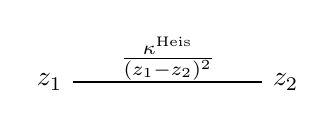
\begin{tikzpicture}
\node at (0,0) {$z_1$};
\node at (3,0) {$z_2$};
\draw[thick] (0.3,0) -- (2.7,0);
\node at (1.5, 0.3) {$\frac{\kappa^{\mathrm{Heis}}}{(z_1-z_2)^2}$};
\end{tikzpicture}
\end{center}

The genus-$0$ bar complex is computed on
$\overline{C}_n(\mathbb{P}^1)$ by logarithmic forms with coefficients
in $a(z_1)\otimes\cdots\otimes a(z_n)$; its differential is the
tree-level chiral factorization residue.
The bar differential uses the logarithmic propagator
$\eta_{12} = d\log(z_1 - z_2)$, which is the unique conformally invariant
1-form with a simple pole along the diagonal (Remark~\ref{rem:why-log-forced}).
It does \emph{not} combine multiplicatively with the OPE propagator
$G(z_1,z_2)=\kappa^{\mathrm{Heis}}(z_1-z_2)^{-2}$; the two objects play distinct roles.
The bar differential applies the chiral residue map:
\begin{equation}\label{eq:heisenberg-bar-residue}
d^{(0)}_{\mathrm{res}}[a \otimes a \otimes \eta_{12}]
= a_{(1)}a
= \kappa^{\mathrm{Heis}} \cdot \mathbf{1},
\end{equation}
because $a_{(0)}a=0$ and the double-pole coefficient is
$a_{(1)}a=\kappa^{\mathrm{Heis}}\mathbf{1}$
(Example~\ref{ex:ope-to-residue} and Proposition~\ref{prop:pole-decomposition}).
The notation $\operatorname{Res}_{D_{12}}$ denotes this chiral residue
operation; it is not the ordinary meromorphic residue of
$\eta_{12}\cdot (z_1-z_2)^{-2}$.
The QFT propagator $G(z,w)=\kappa^{\mathrm{Heis}}/(z-w)^2$ is a separate contraction kernel
for Wick contractions; it does not enter the bar differential.

\section{The free boson at genus~\texorpdfstring{$1$}{1}}

The tadpole diagram (self-contraction on an elliptic curve
$E_\tau = \mathbb{C}/(\mathbb{Z} + \tau\mathbb{Z})$) gives:
\begin{equation}
A_{\text{tadpole}}^{(E_\tau)}
= \kappa^{\mathrm{Heis}}\,G_2(\tau),\qquad
G_2(\tau):=\sideset{}{'}\sum_{(n,m) \in \mathbb{Z}^2}
\frac{1}{(n + m\tau)^2}
= \frac{\pi^2}{3}E_2(\tau),
\end{equation}
with the Eisenstein normalization of
Theorem~\ref{thm:heisenberg-genus-one-complete}.  The modular anomaly
$E_2(-1/\tau) = \tau^2 E_2(\tau) + 6\tau/(\pi i)$
is the one-loop quantum correction to modularity, proportional
to~$\kappa^{\mathrm{Heis}}$.

\begin{center}
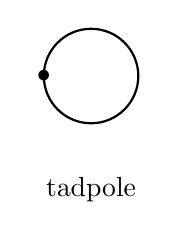
\begin{tikzpicture}[scale=1.2]
\node at (0,0) {$\bullet$};
\draw[thick] (0,0) arc (180:540:0.5);
\node at (0.5, -1.2) {tadpole};
\end{tikzpicture}
\end{center}

In the modular bar complex this trace is not a new
$d^{(0)}$-differential.  The Heisenberg cubic vertex vanishes, so
$K_{1,1}^{\mathcal{H}}=0$ in the stable-graph recursion; the
genus-$1$ scalar comes from the same binary double-pole class
transported through the Hodge line:
\[
\mathrm{obs}_1(\mathcal{H}_{\kappa^{\mathrm{Heis}}})
= \kappa^{\mathrm{Heis}}\lambda_1,\qquad
F_1(\mathcal{H}_{\kappa^{\mathrm{Heis}}})
= \kappa^{\mathrm{Heis}}\!\int_{\overline{\mathcal{M}}_{1,1}}\lambda_1
= \frac{\kappa^{\mathrm{Heis}}}{24}.
\]

\subsection{Loop-genus correspondence}

\begin{theorem}[Loop-genus correspondence; \ClaimStatusProvedElsewhere{} \cite{costello-renormalization}]
\label{thm:loop-genus-correspondence}
\textup{(}\emph{quadrant} graph-combinatorial \textup{(}cited\textup{)},
\emph{presentation} ribbon graph thickening to a closed surface,
\emph{level} 5 of the Beilinson tower \textup{(}stable genus on
$\overline{\mathcal{M}}_{g,n}$\textup{)}, \emph{hypothesis package}
connected ribbon graph with prescribed face count
$F$.\textup{)}
A connected Feynman diagram $\Gamma$ with $V$ vertices, $E$ edges,
and $F$ faces has loop number $L = E - V + 1$. The genus of the
ribbon graph satisfies
$\chi = V - E + F = 2 - 2g$, hence $g = (L + 1 - F)/2 \leq L/2$,
with equality when $F = 1$.
\end{theorem}

The genus in $\bar{B}^{(g)}$ is the stable-curve genus.  In a ribbon
model it is bounded by graph loop number as above, but the
modular characteristic of the Heisenberg theory is linear in the
level:
\[
\mathrm{obs}_g(\mathcal{H}_{\kappa^{\mathrm{Heis}}})
= \kappa^{\mathrm{Heis}}\lambda_g,\qquad
F_g(\mathcal{H}_{\kappa^{\mathrm{Heis}}})
=\kappa^{\mathrm{Heis}}\lambda_g^{\mathrm{FP}}
\]
on the uniform-weight scalar lane (Theorem~\ref{thm:genus-universality}).
Thus the bar genus filtration is not weighted by
$(\kappa^{\mathrm{Heis}})^g$.

\section{One-loop partition function}

The zero-mode-normalised, zeta-regularised Gaussian determinant of the
free boson on $E_\tau$ is
$Z_{E_\tau} = (\mathrm{Im}\,\tau)^{-1/2} |\eta(\tau)|^{-2}$,
which is modular invariant as a density on $\mathcal{M}_{1,0}$.
This is the analytic determinant-line amplitude of the free theory.
The bar complex does not identify this function with a homology group
or construct it as a field-space measure integral. Its vacuum line is
$H^0(\bar{B}^{(1)}(\mathcal{H}_{\kappa^{\mathrm{Heis}}}))=\mathbb{C}$,
and its scalar anomaly is
$F_1(\cA)=\kappa(\cA)\deg(\lambda_1)=\kappa(\cA)/24$
(Theorems~\ref{thm:genus-universality}
and~\ref{thm:explicit-theta}).

\section{The bar complex and the path integral}

\begin{conjecture}[Gaussian BV--bar comparison for the free boson;
\ClaimStatusConjectured]\label{conj:v1-bar-cobar-path-integral-heisenberg}
\textup{(}\emph{quadrant} Open, \emph{presentation} bar / twisting
coalgebra at level~$2$ compared with chain-level BV at level~$1$,
\emph{level} 1 $\to$ 2 of the Beilinson tower with descent to clutching
on $\overline{\mathcal{M}}_{g,n}$ at level~$5$,
\emph{hypothesis package} Heisenberg level
$\kappa^{\mathrm{Heis}} \neq 0$; zero-mode reduction; compatibility
with sewing maps and Hodge classes $\lambda_g$; this conjecture is a
level-$2$ chain-level comparison and does not subsume the
Theorem~\ref{thm:swiss-cheese-chiral-DT-feynman} mechanism for the
holographic uplift to the bulk.\textup{)}
For the Heisenberg vertex algebra $\mathcal{H}_{\kappa^{\mathrm{Heis}}}$
\textup{(}free boson at nonzero Heisenberg level\textup{)} on a
compact Riemann surface $\Sigma_g$ of genus~$g \geq 0$, there is a
genus-filtered comparison morphism
\[
\Phi_g^{\mathrm{Heis}}\colon
C^\bullet_{\mathrm{BV,red}}(\Sigma_g;\mathcal{H}_{\kappa^{\mathrm{Heis}}})
\longrightarrow
\bar{B}_{\mathrm{geom}}^{(g)}(\mathcal{H}_{\kappa^{\mathrm{Heis}}})
\]
from the zero-mode-reduced Gaussian BV complex to the geometric bar
complex.  It sends Wick contraction classes to the chiral residue
class \eqref{eq:heisenberg-bar-residue}, sends the normalized
partition function to the generator of the vacuum line
$H^0=\mathbb{C}$, and induces the cohomology groups of
Theorem~\ref{thm:heisenberg-higher-genus}.
\end{conjecture}

\begin{remark}[Constraints on the Gaussian comparison]
Any morphism
$\Phi_g^{\mathrm{Heis}}$ in
Conjecture~\ref{conj:v1-bar-cobar-path-integral-heisenberg} must
satisfy the following three conditions. First, it must induce the
cohomology computed in Theorem~\ref{thm:heisenberg-higher-genus}:
\[
H^n(\bar{B}^{(g)}(\mathcal{H}_{\kappa^{\mathrm{Heis}}})) = \begin{cases}
\mathbb{C} & n = 0, \\
\mathbb{C}^{2g} & n = 1, \\
\mathbb{C} \oplus \mathbb{C} \cdot c_{\kappa^{\mathrm{Heis}}}^{(g)} & n = 2, \\
0 & n > 2.
\end{cases}
\]
Second, after removing the zero-mode volume, the normalized Gaussian
partition function must land on the generator of the vacuum line
$H^0=\mathbb C$, and the Wick contraction
\[
\langle J(z)J(w)\rangle=\frac{\kappa^{\mathrm{Heis}}}{(z-w)^2}
\]
must map to the residue class
$c_{\kappa^{\mathrm{Heis}}}^{(g)}$. Third, the $2g$ zero-mode
classes of the BV complex must map isomorphically to
$H^1(\Sigma_g,\mathbb C)$ in bar degree~$1$.

For free fields the reduced bar complex is already proved
quasi-isomorphic to the chain-level BV complex
(Proposition~\ref{prop:bar-bv-free-fields}). The remaining assertion
is compatibility with the genus-completed modular bar structure, the
sewing maps, and the Hodge classes $\lambda_g$.
\end{remark}

\begin{conjecture}[Bar-cobar as worldsheet path integral: general case; \ClaimStatusConjectured]\label{conj:v1-bar-cobar-path-integral}
\textup{(}\emph{quadrant} Open, \emph{presentation} bar / twisting
coalgebra compared with BV factorisation algebra,
\emph{level} 1 $\to$ 2 of the Beilinson tower,
\emph{hypothesis package} chiral algebra $\cA$ on $\Sigma_g$ with a
chosen BV/BRST factorisation model of local observables
$\mathcal{F}_{\cA, g}$; nonlinear OPE vertices admitting Arnold-sign
and FM boundary-orientation compatibility; the conjecture compares
chain-level computational presentations and does not displace the
Theorem~\ref{thm:swiss-cheese-chiral-DT-feynman} explanatory
mechanism.\textup{)}
Let $\cA$ be a chiral algebra on $\Sigma_g$ equipped with a
BV/BRST factorization model of local observables
$\mathcal{F}_{\cA,g}$.  There is a genus-completed
$L_\infty$ comparison morphism
\[
\Phi_g^{\mathrm{BV/bar}}\colon
\mathcal{F}_{\cA,g}\longrightarrow \bar{B}^{\mathrm{ch},g}(\cA)
\]
whose genus-$0$ anomaly-free Kac--Moody specialization is the
quasi-isomorphism of Theorem~\ref{thm:brst-bar-genus0} and whose
degree-$2$ scalar projection is
$\Theta_\cA^{\leq 2}=\kappa(\cA)\cdot\eta\otimes\Lambda$
as in Theorem~\ref{thm:explicit-theta}.  The missing datum is the
construction of $\Phi_g^{\mathrm{BV/bar}}$ for nonlinear OPE vertices,
with the Arnold signs and Fulton--MacPherson boundary orientations
compatible with the stable-graph MC equation.
\end{conjecture}

\begin{remark}[Shadow depth in the Feynman picture]
\label{rem:feynman-depth-decomposition}
The loop-genus correspondence of
Theorem~\ref{thm:loop-genus-correspondence} supplies only a graph
bound.  The invariant controlling this monograph is the algebraic
shadow depth
\[
r_{\max}(\cA)=\sup\{r\geq 2:\cA^{\mathrm{sh}}_{r,0}\neq 0\},
\]
not the loop order of a chosen perturbative model
(Definition~\ref{def:generating-depth} and
Theorem~\ref{thm:shadow-archetype-classification}).  A Feynman drawing
of $S_r(\cA)$ should be read as a stable-graph contact term of
arity~$r$, not as a literal connected $(r-1)$-loop amplitude.
\end{remark}

\begin{remark}[Shadow-Feynman dictionary]
\label{rem:feynman-shadow-loop-dictionary}
\index{shadow tower!Feynman dictionary|textbf}
\index{Feynman diagram!shadow correspondence}
Under the Feynman-bar mnemonic
(Remark~\ref{rem:feynman-bar-bridge}), the shadow coefficient
$S_r(\cA)$ is the degree-$r$ stable-graph vertex in the MC tower.
The proved census gives the following exact truncation data
(Table~\ref{tab:shadow-invariants-landscape}):
\begin{itemize}
\item Class~$\mathsf{G}$ (Heisenberg): tower terminates at
 $r_{\max} = 2$; $S_r = 0$ for $r \geq 3$.
\item Class~$\mathsf{L}$ (affine Kac--Moody): tower terminates at
 $r_{\max} = 3$; the cubic shadow is the Lie bracket and
 $S_r = 0$ for $r \geq 4$.
\item Class~$\mathsf{C}$ (standard $\beta\gamma_\lambda$ line):
 $r_{\max} = 4$ with
 $S_2 = 6\lambda^2 - 6\lambda + 1$, $S_3 = 0$,
 $S_4 = -5/12$, and $S_r = 0$ for $r \geq 5$.
\item Class~$\mathsf{M}$ (Virasoro, $\Walg_N$): tower extends to
 $r_{\max} = \infty$; for Virasoro,
 $S_2=c/2$, $S_3=2$,
 $S_4=10/[c(5c+22)]$, and
 $S_5=-48/[c^2(5c+22)]$.
\end{itemize}
These are bar-degree and stable-vertex statements.  A physical loop
interpretation is an additional model-dependent realization, not the
definition of the invariant.
\end{remark}

\begin{remark}[Structural cross-references]
\label{rem:feynman-anchors}
\index{Feynman entry point!structural anchors}
The Feynman picture intersects the main structural spine at three
points:
\begin{enumerate}[label=\textup{(W\arabic*)}]
\item \emph{Universal conductor.} The free-boson partition function
 has vacuum line $H^0=\mathbb{C}$ after zero-mode normalization.
 Its scalar genus-$g$ obstruction is
 $\mathrm{obs}_g(\mathcal{H}_\kappa)=\kappa\,\lambda_g$,
 and the genus-$1$ scalar free energy is
 $F_1(\mathcal{H}_\kappa)=\kappa/24$.  This is the
 per-family instance of the
 universal conductor identity $\kappa(\cA) = -c_{\mathrm{ghost}}(\BRST(\cA))$
 of Chapter~\ref{chap:universal-conductor}; the BRST nilpotence
 condition $c_{\mathrm{matter}} + c_{\mathrm{ghost}} = 0$ is
 precisely the path-integral statement that the one-loop
 anomaly cancels.
\item \emph{Climax identity.} The bar differential
 $d^{(0)}_{\mathrm{res}}[a \otimes a \otimes \eta_{12}]
 = \kappa^{\mathrm{Heis}} \cdot \mathbf{1}$
 of \eqref{eq:heisenberg-bar-residue} is the Heisenberg
 Feynman-rule realisation of the climax identity
 $d_{\mathrm{bar}} = \mathrm{KZ}^*(\nabla_{\mathrm{Arnold}})$
 of Chapter~\ref{ch:climax-theorem}: the Arnold form
 $\eta_{12}$ pulled back through the KZ map supplies the logarithmic
 collision form, and the double-pole OPE supplies the scalar
 residue $\kappa^{\mathrm{Heis}}$.
\item \emph{Cross-volume bridge.} The all-genera Heisenberg
 conjecture (Conjecture~\ref{conj:v1-bar-cobar-path-integral-heisenberg})
 is a Vol~I level-2 chain-level input
 (\emph{quadrant} Open, \emph{presentation} bar / twisting coalgebra,
 \emph{level} 2 of the Beilinson tower,
 \emph{hypothesis package} Heisenberg level
 $\kappa^{\mathrm{Heis}} \neq 0$ + zero-mode reduction).
 The mechanism by which this level-2 datum produces a
 $3$d holomorphic-topological bulk is \emph{not} the bar direction
 alone: it is the chiral Deligne--Tamarkin theorem
 (Theorem~\ref{thm:swiss-cheese-chiral-DT-feynman} below;
 Vol~I `chapters/theory/chiral_center_theorem.tex'
 Theorem~\ref{thm:chiral-deligne-tamarkin}), which constructs the
 universal Swiss-cheese pair
 $(\mathrm{C}^\bullet_{\mathrm{ch}}(A_b, A_b),\, A_b)$
 carrying the action of the open colour ($A_b$) on the closed
 colour ($\mathrm{C}^\bullet_{\mathrm{ch}}(A_b, A_b) =
 Z^{\mathrm{der}}_{\mathrm{ch}}(A_b)$) over the
 $\SCchtop$-operad of Voronov~\cite{Voronov99} +
 chiral analogue of Kontsevich--Soibelman~\cite{KS00}.
 The bar coalgebra $B(A_b)$ is the level-2 \emph{computational model}
 used to compute and present this Swiss-cheese pair; it is not the
 source of the dimensional uplift.
 Vol~II's universal celestial holography on the closed colour
 (Vol~II Theorem~\ref{V2-thm:universal-holography-master}) is
 the level-3 holographic equivalence corresponding to the bulk;
 the comparison passes through Swiss-cheese, not through the
 bar alone.
 For K3-fibered Class~A threefolds this further descends, via the
 Vol~III two-stage CY-to-chiral output
 $\Phi_3^{(\Sigma_2, C)} = \SpCh_{\Sigma_2, C} \circ \PhiFA_3$ at the
 K3 reference curve $C = E_\tau$, to the BPS-counting partition
 function, with the conditional conductor comparison to the proved
 Borcherds weight $\kappa_{\mathrm{BKM}}(\Phi_N) = c_N(0)/2$ on the
 five verified Borcherds families $N \in \{1,2,3,4,6\}$.
\end{enumerate}
\end{remark}

\begin{theorem}[Swiss-cheese / chiral Deligne--Tamarkin;
\ClaimStatusProvedElsewhere]
\label{thm:swiss-cheese-chiral-DT-feynman}
\index{Swiss-cheese operad!chiral Deligne--Tamarkin|textbf}
\index{chiral Deligne--Tamarkin theorem!explanatory mechanism|textbf}
\textup{(}\emph{quadrant} Open, \emph{presentation} Swiss-cheese pair,
\emph{level} 1 $\to$ 3 of the Beilinson tower, \emph{hypothesis package}
local $\Ainf$-chiral algebra $A_b$ on a tangential log curve
$(X, D, \tau)$ with completed conformal-weight topology and finite
chiral residue at every double-point collision.\textup{)}
Let $A_b$ be a local $\Ainf$-chiral algebra. The universal local
chiral Swiss-cheese pair
\[
U(A_b) = \bigl(\mathrm{C}^\bullet_{\mathrm{ch}}(A_b, A_b),\, A_b,\,
\{\mu^{\mathrm{univ}}_{p;q}\}\bigr)
\]
is terminal in the category of local $\SCchtop$-pairs over $A_b$:
the closed colour $\mathrm{C}^\bullet_{\mathrm{ch}}(A_b, A_b)
= Z^{\mathrm{der}}_{\mathrm{ch}}(A_b)$ acts on the open colour $A_b$
through the chiral Swiss-cheese operations
$\mu_{p;q}$ \textup{(}$p$ closed, $q$ open inputs\textup{)}; the
open colour does not act back on the closed colour. For any local
$\SCchtop$-pair $(B, A_b, \{\mu_{p;q}\})$ over $A_b$ with continuous
operations there is a unique morphism
$\Phi \colon (B, A_b, \mu) \to U(A_b)$ over $\mathrm{id}_{A_b}$.
\end{theorem}

\begin{proof}[Citation]
This is Vol~I `chapters/theory/chiral\_center\_theorem.tex'
Theorem~\ref{thm:chiral-deligne-tamarkin}, the chiral analogue of
the Voronov Swiss-cheese formality theorem~\cite{Voronov99} and the
Kontsevich--Soibelman Deligne conjecture~\cite{KS00}. The proof
constructs $\Phi(b)(a_1, \ldots, a_n; \lambda_1, \ldots, \lambda_{n-1})
= (-1)^{|b|} \mu_{1;n}(b; a_1, \ldots, a_n; \lambda_1, \ldots,
\lambda_{n-1})$ on $n-1$ open-sector spectral variables.
\end{proof}

\begin{remark}[The Swiss-cheese pair is the explanatory mechanism;
the bar is computational]
\label{rem:swiss-cheese-not-bar-feynman}
\index{bar-computational!corrected!bar is computational|textbf}
\index{dimensional uplift!Swiss-cheese mechanism|textbf}
The dimensional uplift from a $2$-real-dimensional chiral algebra
on a curve $X$ to a $3$-real-dimensional holomorphic-topological
bulk on $X \times \bR_{\ge 0}$ is a property of the
\emph{Swiss-cheese pair} $(Z^{\mathrm{der}}_{\mathrm{ch}}(A_b),
A_b)$ produced by the chiral Deligne--Tamarkin terminal-object
construction (Theorem~\ref{thm:swiss-cheese-chiral-DT-feynman}).
The extra topological dimension is the universal normal-collar
direction of the codimension-one boundary condition forced by the
centre construction; it is not produced by iterating the bar
construction on $A_b$ alone.

The bar coalgebra $B(A_b) = T^c(s^{-1} \bar{A}_b)$ is
$E_1$-coassociative on the curve geometry: a single primitive
twisting coalgebra over the chiral associative operad. It is a
chain-level computational model
that resolves $A_b$ for the purpose of computing
$\mathrm{C}^\bullet_{\mathrm{ch}}(A_b, A_b)$ via
$\mathrm{Hom}_{\mathrm{ch}}(B(A_b), A_b)$, but the closed colour
of the holographic pair is the chiral Hochschild cochain complex,
not the bar coalgebra. Drawings such as
Construction~\ref{constr:feynman-stable-graph}, the genus-$g$
Feynman expansions of equation~\eqref{eq:feyn-W15-1loop-logZ}, and
the BPHZ-shape $A_\infty$ relations of
Section~\ref{sec:bphz-ainfinity} are visualisations of the bar
side of this resolution; the holographic mechanism that lifts $A_b$
to a $3$d HT theory is the universal property of the Swiss-cheese
pair, not the bar differential.
\end{remark}

\begin{remark}[Scope of the bar-path-integral comparison]\label{rem:bar-path-integral-scope}
Conjecture~\ref{conj:v1-bar-cobar-path-integral-heisenberg} records
the bar-complex/path-integral comparison for
$\mathcal{H}_{\kappa^{\mathrm{Heis}}}$ at all genera.  For interacting
chiral algebras $\cA$, only the genus-$0$ algebraic BRST/bar
comparison on the Kac--Moody locus and the local binary/ternary
reduction package are proved in this volume
(Theorem~\ref{thm:brst-bar-genus0}); the all-genera comparison is
Conjecture~\ref{conj:v1-bar-cobar-path-integral}.

All Arnold-relation and sign checks occur in the ordered
$E_1$ lift before averaging.  The symmetric modular class is obtained
after quotienting labelled configurations by the symmetric group; the
stable-graph automorphism denominators in
Construction~\ref{constr:feynman-stable-graph} belong to this
averaged surface.  The path-integral comparison is also separate from
the three structural identifications in the spine of the monograph:
$\Omega^{\mathrm{ch}}\bar{B}^{\mathrm{ch}}(\cA)\simeq\cA$ is
bar-cobar inversion, $\mathbb{D}_{\Ran}\bar{B}_X(\cA_i)\simeq\cA^!$
is Verdier duality, and
$Z^{\mathrm{der}}_{\mathrm{ch}}(\cA)$ is governed by chiral
Hochschild cochains (Convention~\ref{conv:three-hochschild}).
\end{remark}
